%%
%% This is file `sample-sigconf.tex',
%% generated with the docstrip utility.
%%
%% The original source files were:
%%
%% samples.dtx  (with options: `sigconf')
%% 
%% IMPORTANT NOTICE:
%% 
%% For the copyright see the source file.
%% 
%% Any modified versions of this file must be renamed
%% with new filenames distinct from sample-sigconf.tex.
%% 
%% For distribution of the original source see the terms
%% for copying and modification in the file samples.dtx.
%% 
%% This generated file may be distributed as long as the
%% original source files, as listed above, are part of the
%% same distribution. (The sources need not necessarily be
%% in the same archive or directory.)
%%
%%%% Proceedings format for most of ACM conferences (with the exceptions listed below) and all ICPS volumes.

%%\documentclass[sigconf]{acmart}

\documentclass[acmconf,authordraft]{acmart}


\usepackage{algpseudocode} 
\usepackage{algorithm}

%%%% As of March 2017, [siggraph] is no longer used. Please use sigconf (above) for SIGGRAPH conferences.

%%%% Proceedings format for SIGPLAN conferences 
% \documentclass[sigplan, anonymous, review]{acmart}

%%%% Proceedings format for SIGCHI conferences
% \documentclass[sigchi, review]{acmart}

%%%% To use the SIGCHI extended abstract template, please visit
% https://www.overleaf.com/read/zzzfqvkmrfzn

%%
%% \BibTeX command to typeset BibTeX logo in the docs
\AtBeginDocument{%
  \providecommand\BibTeX{{%
    \normalfont B\kern-0.5em{\scshape i\kern-0.25em b}\kern-0.8em\TeX}}}

%% Rights management information.  This information is sent to you
%% when you complete the rights form.  These commands have SAMPLE
%% values in them; it is your responsibility as an author to replace
%% the commands and values with those provided to you when you
%% complete the rights form.
\setcopyright{acmcopyright}
\copyrightyear{2018}
\acmYear{2018}
\acmDOI{10.1145/1122445.1122456}

%% These commands are for a PROCEEDINGS abstract or paper.
\acmConference[Woodstock '18]{Woodstock '18: ACM Symposium on Neural
  Gaze Detection}{June 03--05, 2018}{Woodstock, NY}
\acmBooktitle{Woodstock '18: ACM Symposium on Neural Gaze Detection,
  June 03--05, 2018, Woodstock, NY}
\acmPrice{15.00}
\acmISBN{978-1-4503-9999-9/18/06}


%%
%% Submission ID.
%% Use this when submitting an article to a sponsored event. You'll
%% receive a unique submission ID from the organizers
%% of the event, and this ID should be used as the parameter to this command.
%%\acmSubmissionID{123-A56-BU3}

%%
%% The majority of ACM publications use numbered citations and
%% references.  The command \citestyle{authoryear} switches to the
%% "author year" style.
%%
%% If you are preparing content for an event
%% sponsored by ACM SIGGRAPH, you must use the "author year" style of
%% citations and references.
%% Uncommenting
%% the next command will enable that style.
%%\citestyle{acmauthoryear}

%%
%% end of the preamble, start of the body of the document source.
\begin{document}

%%
%% The "title" command has an optional parameter,
%% allowing the author to define a "short title" to be used in page headers.
\title{Concise Description of Telecom Service Use Through Concept Chains}

%%
%% The "author" command and its associated commands are used to define
%% the authors and their affiliations.
%% Of note is the shared affiliation of the first two authors, and the
%% "authornote" and "authornotemark" commands
%% used to denote shared contribution to the research.
\author{Ants Torim}
\email{ants.torim@taltech.ee}
\author{Sadok Ben Yahia}
\email{sadok.ben@taltech.ee}
\author{Kristo Raun}
\email{kristo.raun@gmail.com}
\affiliation{%
  \institution{Tallinn University of Technology, Department of Software Science}
  \streetaddress{Akadeemia tee 15a}
  \city{Tallinn}
  \state{Estonia}
  \postcode{12618}
}





%%
%% The abstract is a short summary of the work to be presented in the
%% article.
\begin{abstract}
Binary data arise naturally in many fields including shopping carts, pass-fail tests, social networks etc. Descriptive data mining aims to discover a concise set of general patterns in these possibly noisy data. An important tool for describing binary data is Formal Concept Analysis (FCA) which describes the data through formal concepts. 
As the full lattice of formal concepts can become large even when dealing with relatively modest amounts of data  there are several methods to  reduce the number of concepts used to describe the data: selecting a subset of ``interesting''  concepts, finding a subset of  concepts that cover the data  fully etc.
In this paper we apply a novel method of concept chain coverage generation to service use data of a telecommunications company. Concept chain coverage aims to cover the data not with single concepts but with chains of related concepts. The aim is not the full coverage but high enough coverage through a concise set of concept chains. We show that a relatively modest set of concept chains (4 to 10) can describe most of the data and that the performance of the algorithm is very acceptable for this case study. 

\end{abstract}

%%
%% The code below is generated by the tool at http://dl.acm.org/ccs.cfm.
%% Please copy and paste the code instead of the example below.
%%
\begin{CCSXML}
<ccs2012>
 <concept>
  <concept_id>10010520.10010553.10010562</concept_id>
  <concept_desc>Computer systems organization~Embedded systems</concept_desc>
  <concept_significance>500</concept_significance>
 </concept>
 <concept>
  <concept_id>10010520.10010575.10010755</concept_id>
  <concept_desc>Computer systems organization~Redundancy</concept_desc>
  <concept_significance>300</concept_significance>
 </concept>
 <concept>
  <concept_id>10010520.10010553.10010554</concept_id>
  <concept_desc>Computer systems organization~Robotics</concept_desc>
  <concept_significance>100</concept_significance>
 </concept>
 <concept>
  <concept_id>10003033.10003083.10003095</concept_id>
  <concept_desc>Networks~Network reliability</concept_desc>
  <concept_significance>100</concept_significance>
 </concept>
</ccs2012>
\end{CCSXML}

\ccsdesc[500]{Computer systems organization~Embedded systems}
\ccsdesc[300]{Computer systems organization~Redundancy}
\ccsdesc{Computer systems organization~Robotics}
\ccsdesc[100]{Networks~Network reliability}

%%
%% Keywords. The author(s) should pick words that accurately describe
%% the work being presented. Separate the keywords with commas.
\keywords{big data, services, formal concept analysis, case study}

%% A "teaser" image appears between the author and affiliation
%% information and the body of the document, and typically spans the
%% page.


%%
%% This command processes the author and affiliation and title
%% information and builds the first part of the formatted document.
\maketitle

\section{Telecom Use Case}

\section{Formal Concept Analysis}

\subsection{Fundamentals of FCA}

 Formal concept analysis (FCA) was introduced by Rudolf Wille in 1982 \cite{wille_restructuring_2009} and has many applications \cite{ganter_formal_2005}. Formal concepts are defined for the formal context (informally, a binary data table) and are characterized their extent and intent.


\begin{definition} 
A context \textbf{K} is a triple (O, I, R) where O is a set of objects and I is a set of attributes (or items) and $ {R \subseteq O \times I} $
\end{definition}

A context \textbf{K} is equivalent to a binary data table $D$. Relation $(o, i) \in R$ means that object $o$ has true value (1) for the attribute $i$ in $D$, other values are False (0). 

\begin{definition} 
For $ A \subseteq G $ and $ B \subseteq M $, define 
\begin{equation}
A'=\bigl\{i \in I \mid (\forall o \in A), (o, i) \in R \bigr\} \ ,
\end{equation}
\begin{equation}
B'=\bigl\{o \in O \mid (\forall i \in B), (o, i) \in R \bigr\} \ ;
\end{equation}
so $A'$ is the set of attributes common to all the objects in A and $B'$ is the set of objects possessing the attributes in B.
\label{def:prim}
\end{definition}

\begin{definition}
A formal concept is any pair $\langle A, B \rangle$ where $A \subseteq O $ and $ B \subseteq I $, $A' = B$ and $B' = A$.
The extent of the concept $\langle A, B \rangle$ is A while its intent is B.
\end{definition}

We can say less formally that a concept is a set of objects together with the  attributes these objects have in common under the restriction that we cannot add an additional attribute without removing an object and we cannot add an additional object without removing an attribute. 
An order $C_1 \leq C_2$  for the concepts $C_1 = \langle A_1, B_1 \rangle$ and $C_2 = \langle A_2, B_2 \rangle$ is defined by the subset relations $A_1 \subseteq A_2$ and $B_2 \subseteq B_1$. It can be shown \cite{davey_introduction_2002} that these concepts form a complete lattice, known as the concept lattice. 

\begin{table}
  \caption{A simple  formal context}
  \label{tab:simplecontext}
  \begin{tabular}{lccccc}
    \toprule
    & a & b & c & d & e\\
    \midrule
    1 & 1 & 1 & 1 & 1 & 0\\
    2 & 1 & 1 & 1 & 0 & 0\\
    3 & 1 & 1 & 1 & 0 & 0\\
    4 & 1 & 0 & 0 & 0 & 1\\
    5 & 1 & 0 & 0 & 1 & 1\\
  \bottomrule
\end{tabular}
\end{table}


In example from Table \ref{tab:simplecontext}   $\langle \{123\}, \{abc\} \rangle \leq \langle \{12345\}, \{a\} \rangle$, while concept $\langle \{5\}, \{de\} \rangle$ has no order relation to previous two.

\subsection{Concept Chains}

In the general theory of ordered sets, ordered set $P$ is a chain if for all $x, y \in P$, either $x \leq y$ or $y \leq x$, that is any two elements of $P$ are comparable. $P$ is an antichain if $x \leq y$ only if $x=y$, that is no two elements of $P$ are comparable \cite{davey_introduction_2002}, \cite{ore_chains_1943}.

Concept chain is a sequence of concepts
\begin{equation}
  (C_1, C_2,..., C_n) = (\langle A_1, B_1 \rangle,\langle A_2,B_2 \rangle,  ..., \langle A_n,B_n \rangle)  \text{ ,where  }  A_i \supset  A_{i+1} \text{ for all } i
\end{equation}

Of course
\begin{displaymath}
A_i \supset A_{i+1} \equiv B_i \subset B_{i+1} \equiv C_i > C_{i+1}
\end{displaymath}

For example, in Table \ref{tab:simplecontext}, we can define a concept chain 
$(\langle \{12345\}, \{a\} \rangle,
 \langle \{123\}, \{ab\} \rangle,  
 \langle \{1\}, \{abcd\} \rangle)$.

As there is an overlap between sequential extents and intents, it useful to concentrate on the differences between extents ($dA_i$) and intents ($dB_i$).

\begin{equation}
dA_k = A_k - A_{k+1}
\end{equation}

\begin{equation}
dB_k = B_k - B_{k-1}
\end{equation}

\begin{equation}
A_k = \bigcup_{i=k}^{n} dA_i
\end{equation}

\begin{equation}
B_k = \bigcup_{i=1}^{k} dB_i
\end{equation}

As there are usually too many objects to describe  individually, it is useful to replace the actual objects in the extent with the size of the extent giving us the following shorter concept chain description:

\begin{displaymath}
 (\langle|A_1|, dB_1 \rangle,\langle |A_2|, dB_2 \rangle,  ..., \langle |A_n|, dB_n \rangle)
\end{displaymath}

So our example concept chain 
$(\langle \{12345\}, \{a\} \rangle,
 \langle \{123\}, \{ab\} \rangle,  \langle \{1\}, \{abcd\} \rangle)$
 can be shortened into
 \begin{displaymath}
 (\langle 5, \{a\} \rangle,
 \langle 3, \{b\} \rangle,  
 \langle 1, \{cd\} \rangle)
 \end{displaymath}.

In summary the concept chain is a sequence of concepts ordered by subset / super-set relations between concept intents and extents. We can reduce the amount of duplication which would occur when describing complete extents and intents and describe the concepts in the chain additively.

\subsection{Context Coverage Problem}

There are different variations for the context covering problem:

\begin{itemize}
  \item To cover the concepts in the formal context fully with concept chains.
  \item To cover the binary relations in formal context / ones in the binary data table fully.
  \item To cover the binary relations in formal context / ones in the binary data table partially.
\end{itemize}

The problem of covering all the concepts in the formal context with concept chains is related to Dilworth's theorem \cite{dilworth_decomposition_1950} which states that for any finite partially ordered set the largest antichain has the same size as the smallest chain decomposition. Therefore the number of concept chains needed to cover the concept lattice equals to the size of the largest antichain in the lattice. As the number of formal concepts can grow exponentially in relation to the size of the formal context the solution to this problem is unlikely to be concise and we won't be dealing with this problem in this article.

The problem of covering all the binary relations in the formal context (ones in the binary data table) is also well known and well researched.  Belkhiter et al introduced a rectangular decomposition of a formal concept [Belkhiter citation]. Belohlavek and Vychodil and later Belohlavek and Trnecka have introduced several approaches for decomposing a binary matrix into a Boolean product of factors \cite{belohlavek_discovery_2010}, \cite{belohlavek_-below_2015}. Later Moukhater and Ben Yahia proposed a method for the extraction of formal concept coverage for the formal context and confirmed that their QualityCover algorithm produces results that are superior to previous approaches \cite{mouakher_qualitycover:_2016}. We will be applying this approach to our case study.

The amount of concepts needed to cover the formal context fully can still be quite large. Therefore we are also reviewing the partial context covering problem, which we define as follows:

\begin{definition}
\label{def_errors}

Given a formal context $ K = (G, M, I)$ and a threshold $\delta$, find the set of concepts $C$, so that for the set of errors $E = \{e \mid e \subseteq I, \forall (A, B) \in C: e \notin (A \times B)  \}$ the number of errors $|E|$ is less than or equal to $\delta$, and the number of concepts, $|C|$, is minimal.

\end{definition}

For example, for the set of concepts \{${(12345, a), (1, abcde)}$\} in Table \ref{tab:simplecontext}  we have $|E|=7$.

This problem is equivalent to $\delta$-approx role mining problem described by Vaidya et al. \cite{vaidya_role_2007} where it is also proven (through transformation to set basis problem) that this problem is NP-complete. Several approaches exist for finding most interesting concepts \cite{kuznetsov_concept_2015}, \cite{kuznetsov_stability_2007}.

We will be using concept chains instead of formal concepts for partial context coverage. Early version of the problem of partial concept chain cover was described by R. Kuusik in 1989 \cite{kuusik_application_1989} as the problem of finding the best branch in the decision tree. The algorithm guaranteed optimal result according to certain measure, but was relatively slow. Some speed improvements were proposed by A. Torim in 2005 \cite{torim_describing_2005} but algorithm remained usable only for small data tables. It also generated only a single concept chain. Therefore we focus here on heuristic approaches. These approaches and algorithms are described by Torim et al \cite{torim_covering_2019}.

\subsection{Algorithms for Generating the Concept Cover}
QualityCover

\subsection{Algorithm for Generating the Concept Chain Cover}

Here we describe shortly the Conformism Lexicographic and Restoration (CLeaR) Sort Algorithm for concept chain generation. Detailed discussion of this algorithm is out of the scope of this article, which focuses on the case study of Telecom data but we provide a short description for completeness sake.

$ConceptChainCover()$ takes a binary data table $D^0$ and returns a sequence of concept chains which leaves $delta$ or less errors (uncovered ones).

\begin{algorithm}
\caption{ConceptChainCover($D^0, \delta$)}
\label{Meta-algorithm}
\begin{algorithmic}
\State $C_{seq} \gets ()$
\State $D \gets D^0$
\While {Number of errors $|E|$ for concepts in $C_{seq}$ covering binary matrix $D$ is smaller than $\delta$ (see def.\ref{def_errors}) }
    \State  $C \gets ConceptChain(CLeaRSort(D, D^0))$ (generate a concept chain from reordered $D$)
    \State Append $C$ into $C_{seq}$
    \State Remove all concepts in $C$ from $D$, that is for all $(A, B) \in C$ remove  $A \times B$ from $I$.
\EndWhile
\State \Return $C_{seq}$
\end{algorithmic}
\end{algorithm}

CLeaR-Sort is based on the FL-Sort algorithm described in \cite{torim_covering_2019}. It reorders the binary data table $D$ so that its upper left corner is filled with ones, corresponding to a concept chain.  It introduces two improvements: it uses conformism instead of frequencies for initial sorting and a restore step that compares the data table $D$, from which the previous concept chains have been removed, with original data table $D_0$ and restores removed ones if they help to create a bigger chain. 


\begin{algorithm}
\caption{CLeaRSort($D$, $D^0$)}
\label{CLeaR-Sort}
\begin{algorithmic}
\State Sort all rows in $D$ by conformism
\State Sort all columns in $D$ by conformism
\State $SortByRows \gets True$
\While {$D \neq D_{old}$}
    \State $D_{old} \gets D$
    \If {$SortByRows$}
        \State Restore the rows of $D$ from $D^0$ 
        \State Sort $D$ lexicographically by rows
    \Else
        \State Restore the columns of $D$ from $D^0$
        \State Sort $D$ lexicographically by columns
    \EndIf
    \State $SortByRows \gets \neg SortByRows$
\EndWhile
\State \Return $D$
\end{algorithmic}
\end{algorithm}

Conformism measure $w(x)$ for an object or an attribute $x$ comes from the theory of monotone systems \cite{vohandu_algorithms_2006} and is defined as

\begin{equation}
w(x) = \sum_{y \in x'}|y'|
\label{ms_weight}
\end{equation}

To restore ones for the $j$-th row from the original data table $D^0_j$ to the row of the current data table $D_j$ we calculate the length of unbroken sequence of ones from left to right.

\begin{equation}
ones(D_j) = max(\{n \mid \forall i \leq n, D_{ji}=1\})
\label{ones}
\end{equation}

Then we find the restore position $r_j$ (if any) up to which we should insert ones from left to right into the row $D_j$. That is to make ones in $D_j$ not yet in unbroken sequence of ones part of such a sequence and through the lexicographic sorting part of the concept chain.

\begin{equation}
r_j = max(\{p \mid   ones(D_j) < \forall p \leq ones(D^0_j)+1, D_{jp}=1\})
\label{restore}
\end{equation}

Restoring ones by columns is defined dually.


This concludes our description of CLeaRSort algorithm. Short description was provided, more detailed description with examples and comparison with alternatives like FL-Sort is outside the scope of this article.

\section{Complete Concept Cover for Telecom Data}
Full lattice has 27475 formal concepts, Quality Cover generates the cover of 534 concepts.

\section{Concept Chain Cover for Telecom Data}

We applied our CLeaR-Sort  concept chain generation algorithm to Telia service usage data. The running time, reported by Pythons $timeit$module and averaged over 7 tries, was $2.28 s \pm 77 ms$ per try. The test was performed on a desktop computer with a 3.50 GHz Intel(R) Core(TM) i5-6600K CPU. The algorithm was set to stop after 90\% of the data table was covered, which occurred after the generation of 19 concept chains. 

\begin{figure}[ht]
  \centering
   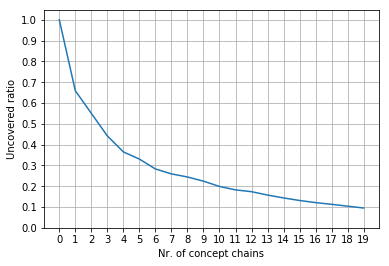
\includegraphics[width=\linewidth]{telia_ccc}
  \caption{How much of the data table is uncovered by generated concept chains.}
  \Description{Uncovered ratios.}
  \label{fig_cc_cover}
\end{figure}

Figure \ref{fig_cc_cover} shows the amount of data table still uncovered for $n$ concept chains.
We can see that the first concept chain covers about 34\% of the data table. First four concept chain cover about 64\% of the data table after which additional concept chains cover add less and less cover. It is similar to elbow method [ref to elbow method] used to find the optimal number of clusters which plots the average distance between objects and their cluster centroids. As the number of clusters increases this distance decreases but the aim is to keep both the number of clusters and the distance low. An elbow point in the distance-nr of clusters curve is the point closest to lower left corner, that is the point where the distance reduction from additional clusters becomes smaller and smaller. In the case of concept chains we have similar tension between the number of chains and data table uncovered. Additional chains cover more data but we want to keep the number of chains reasonably low. An elbow point on the curve represents a reasonable compromise and for this case study this seems to be four concept chains.

To cover 80\% of the concept lattice 10 concept chains are needed by CLeaR-Sort. This compares favourably to simpler FL-Sort algorithm \cite{torim_covering_2019} which needed 13 chains for 80 \% coverage. Detailed comparison of those algorithms is however outside the scope of this article.

Let us now examine four first concept chains in detail, starting with the first chain, that covers 34\% of the service data. The chains $cc_1$, $cc_2$, $cc_3$ and $cc_4$ are shown below. The services are anonymized and shown only through their codes (s$i$). Concept chains are shown from the first concept to the last concept in the $\langle|A_1|, dB_1 \rangle$ format. Numbers show the extent size of the concept which decreases as the chain grows.  For example the second concept in the chain $\{s11, s56\}$ has the extent size of 316.

$cc_1 = $
$\langle 411, {s11} \rangle$,
$\langle 316, {s56} \rangle$,
$\langle 315, {s18} \rangle$,
$\langle 297, {s64} \rangle$,
$\langle 158, {s44} \rangle$,
$\langle 157, {s43} \rangle$,
$\langle 146, {s65} \rangle$,
$\langle 114, {s61} \rangle$,
$\langle 108, {s13} \rangle$,
$\langle 43, {s58} \rangle$,
$\langle 35, {s10} \rangle$,
$\langle 31, {s35} \rangle$,
$\langle 11, {s51} \rangle$,
$\langle 8, {s50} \rangle$,
$\langle 5, {s23} \rangle$,
$\langle 3, {s9} \rangle$,
$\langle 2, {s63, s36, s41} \rangle$,
$\langle 1, {s22, s21, s66} \rangle$



The coverage of 34 \% by the first concept chain can be compared to the case study with data about students passing or failing  courses \cite{torim_covering_2019}, where first concept chain had   74\% coverage. This data was very well suited to concept chain approach as students rank according to their ability and courses according to their difficulty forming a natural chain.

We can describe our first concept chain as having a short and thick head - services 11 to 64 - and a long thin tail composed of the services 58 to 22. The thin tail contributes relatively little to the total coverage of the chain and we can concentrate on  head. This pattern repeats itself over all four concept chains.

411 customers use service 11, 316 customers use services 11 and 56, 315 customers use services 11, 56 and 18 etc.

Concept chains 2, 3 and 4 are given below.
\\
$cc_2 = $
$\langle 337, {s35} \rangle$,
$\langle 286, {s61} \rangle$,
$\langle 95, {s9} \rangle$,
$\langle 53, {s44} \rangle$,
$\langle 52, {s43} \rangle$,
$\langle 33, {s10} \rangle$,
$\langle 20, {s41} \rangle$,
$\langle 16, {s65, s64} \rangle$,
$\langle 5, {s51} \rangle$,
$\langle 2, {s27, s25} \rangle$,
$\langle 1, {s22, s50, s23, s48} \rangle$.
\\
$cc_3 = $
$\langle 388, {s13} \rangle$,
$\langle 374, {s56, s18} \rangle$,
$\langle 158, {s21} \rangle$,
$\langle 45, {s23} \rangle$,
$\langle 31, {s58} \rangle$,
$\langle 10, {s9} \rangle$,
$\langle 9, {s61} \rangle$,
$\langle 3, {s22, s32} \rangle$,
$\langle 1, {s43, s51, s44, s12, s27, s50} \rangle$.
\\
$cc_4 = $
$\langle 386, {s64} \rangle$,
$\langle 266, {s10} \rangle$,
$\langle 241, {s65} \rangle$,
$\langle 119, {s44} \rangle$,
$\langle 117, {s43} \rangle$,
$\langle 18, {s66} \rangle$,
$\langle 4, {s48} \rangle$,
$\langle 3, {s32} \rangle$,
$\langle 2, {s23, s57, s26, s21} \rangle$,
$\langle 1, {s45, s31, s34} \rangle$.
\\
The set of four concept chains is certainly a concise and human usable description comparing favourably to 534 concepts generated by the QualityCover which itself compares favourably to 27475 concepts in the full lattice. Of course here we are dealing with partial cover vs full cover vs full lattice.

What could be the practical use cases within the services ecosystem for these concept chains? For service usage data they seem to describe typical evolution paths for different client types. For example, in the fourth concept chain ($cc_4$) we can see that from the 266 customers that use both services 64 and 10 a large subset of 241 customers also use service 65. That can form a basis for a recommendation system: if we have customers that use services 64 and 10 then we can recommend and market the service 65 to them. The advantage over traditional recommendation systems would be the concise white box nature of concept chains making them usable for human decision making.

Describing the evolution path is also an advantage of concept chains that single concepts lack as they just state that a certain set of customers use certain services. 

As we can see our CLeaR-Sort algorithm provides an acceptable partial coverage with a concise set of concept chains that help us understand the customer evolution paths within the services ecosystem.


\section{Conclusions}

We applied our method for finding the concept chain cover for the data about telecommunications service use. The results were significantly more concise than the binary relation coverage generated by QualityCover algorithm which has compared favourably against other such methods \cite{mouakher_qualitycover:_2016}. It is important to note that concept chain cover is only partial while QualityCover provides full cover. With our previous  case study about student course completion \cite{torim_covering_2019} this seems to confirm that the method for generating concept chain cover is of interest and useful in different fields. In the ecosystem of telecommunications services it can illuminate various service usage evolution paths.

\bibliographystyle{ACM-Reference-Format}
\bibliography{medes_bib}

\end{document}
\endinput
%%
%% End of file `sample-sigconf.tex'.
